
%% inicio, la clase del documento es iccmemoria.cls
\documentclass{iccmemoria}
\setcounter{secnumdepth}{3} %%Cantidad maxima de subsecciones enumeradas
\newcommand{\grad}{$^{\circ}$}
%\usepackage[utf8]{inputenc} % Caracteres con acentos.
%%\usepackage{enumitem}
\usepackage[inline]{enumitem}

%paquetes para las tablas
\usepackage{color}
\usepackage{colortbl}
\usepackage{multicol}
\usepackage{multirow}
\usepackage{booktabs}
\usepackage{tabularx}

\usepackage{algorithm}
\usepackage[noend]{algpseudocode}
\usepackage{amssymb, amsmath, amsbsy}


%---- Paquete para aliniación de texto verticalmente dentro de tablas
\usepackage{array}
%---- Paquetes para los pies de las tablas
\usepackage{caption}
\usepackage{subcaption}

\definecolor{skyblue6}{rgb}{.2, .6, .8}
\definecolor{firebrick}{rgb}{.7, .13, .13}
\definecolor{blueice}{rgb}{.85, .96, .94}
\definecolor{lightcopper}{rgb}{.93, .76, .58}

%% datos generales y para la tapa
\titulo{Gestión de fondos para actividades estudiantiles conducidas por CCAA o la Fedeut Curicó en acuerdo a la RU N\grad 2083 de 2017}
\author{Yorch Sepúlveda Manríquez}
\supervisor{Rodrigo Paredes Moraleda}
\informantes
	{Renzo Angles Rojas}
	{Ruth Garrido Orrego}
\adicional{(sólo por si se necesita agregar algún otro profesor)}
\director{Profesor del ramo Memoria de Título}
\date{Julio, 2019}

%% inicio de documento
\begin{document}

%% crea la tapa
\maketitle

%% dedicatoria
\begin{dedicatory}
Dedicado a Patricia Manríquez Lisboa y Sergio Sepúlveda Leal, mis padres.
\end{dedicatory}

%% agradecimientos
\subfile{Agradecimientos}

%% indices
\tableofcontents
\listoffigures
\listoftables

%% resumen
\subfile{Resumen}

%% abstract

%% contenido del primer capítulo
\chapter{Introducción}
    \label{sec:Intro}
	\subfile{Capitulo1/1_Introduccion}

	\section{Contexto del proyecto}
	\label{sec:Contexto}
	\subfile{Capitulo1/1.1_Contexto}

	\section{Definición del problema}
	\label{sec:Problema}
	\subfile{Capitulo1/1.2_Definicion_Problema}

	\section{Presentación de la solución}
	\label{sec:Solucion}
	\subfile{Capitulo1/1.3_Presentacion_Solucion}

	\section{Objetivos}
	\label{sec:Objetivos}
	\subfile{Capitulo1/1.4_Objetivos}

	\section{Alcances}
	\subfile{Capitulo1/1.5_Alcances}

	\section{Limitaciones}
	\subfile{Capitulo1/1.6_Limitaciones}

	\section{Proyectos similares}
	\subfile{Capitulo1/1.7_Proyectos_Similares}

	\section{Descripción de contenidos}
	\subfile{Capitulo1/1.8_Descripcion_Contenidos}

%% contenido del segundo capítulo
\chapter{Antecedentes}
\subfile{Capitulo2/2_Introduccion}

	\section{Conceptos}
	\label{sec:Conceptos}
	\subfile{Capitulo2/2.1.1_Conceptos}

	\section{Tecnologías utilizadas}
	\label{sec:Tecnologias}
		\subfile{Capitulo2/2.2_Tecnologias_Utilizadas}
		\subsection{Frameworks}

		\subfile{Capitulo2/2.2.1_Framework}
		\subsection{Bibliotecas}

		\subfile{Capitulo2/2.2.2_Bibliotecas}
		
	\section{Metodología de desarrollo de software}
		\subfile{Capitulo2/2.3_Metodologia_desarrollo}

	\section{Metodología ágil}
	\subfile{Capitulo2/2.4_Metodologia_Agil}

		\subsection{Scrum}
		\subfile{Capitulo2/2.4.1_Scrum}

		\subsection{Roles}
		\label{sec:Roles}
		\subfile{Capitulo2/2.4.2_Roles}

		\subsection{Aptitudes requeridas}
		\subfile{Capitulo2/2.4.3_Aptitudes}

		\subsection{Artefactos}
		\label{sec:Artefactos}
		\subfile{Capitulo2/2.4.4_Artefactos}
		
		\subsection{Reuniones}
		\label{sec:Reuniones}
		\subfile{Capitulo2/2.4.5_Reuniones}
		
		\subsection{Ciclo de vida}
		\subfile{Capitulo2/2.4.6_Ciclo_de_vida}

		\subsubsection{El proyecto}
		\label{sec:Proyecto}
		\subfile{Capitulo2/2.4.7_Proyecto}

		\subsubsection{Las fases}
		\label{sec:Fases}
		\subfile{Capitulo2/2.4.8_Fases}

		\subsection{Documentación}
		\label{sec:Documentacion}
		\subfile{Capitulo2/2.4.9_Documentacion}

	\section{Validación de la aplicación}
		\subfile{Capitulo2/2.5_Pruebas}

	\section{Herramientas de planificación}
		\subfile{Capitulo2/2.6_HerramientasPlanificacion}
	
%% contenido del tercer capítulo
\chapter{Metodología utilizada}
\subfile{Capitulo3/3_Introduccion}

	\section{Estudio del entorno}
	\subfile{Capitulo3/3.1_Entorno}

		\subsection{Las personas}
		\subfile{Capitulo3/3.1.1_Personas}

		\subsection{La aplicación}
		\subfile{Capitulo3/3.1.2_Aplicacion}

		\subsection{Las herramientas}
		\subfile{Capitulo3/3.1.3_Herramientas}
	
	\section{La metodología}
	\subfile{Capitulo3/3.2_Metodologia}
		\subsection{Roles}
		\subfile{Capitulo3/3.2.1_Roles}

		\subsection{El proceso}
		\subfile{Capitulo3/3.2.2_Proceso}

			\subsubsection{El proyecto}
			\subfile{Capitulo3/3.2.2.1_Proyecto}

			\subsubsection{Iteraciones del proyecto}
			\label{sec:Iteracion}
			\subfile{Capitulo3/3.2.2.2_Iteracion}

			\subsubsection{Reuniones}
			\subfile{Capitulo3/3.2.2.3_Reuniones}

		\subsection{Cómo se trabajó}
		\subfile{Capitulo3/3.2.3_Trabajo}
	
%% contenido del Cuarto capítulo
\chapter{Características del sistema}
\label{sec:Caracteristica_Sistema}
\subfile{Capitulo4/4_Introduccion.tex}

	\section{Aspectos generales}
	\subfile{Capitulo4/4.1_AspectosGenerales}

	\section{Modelos de contexto de solicitudes}
	\label{sec: Contexto_Solicitud}
	\subfile{Capitulo4/4.2_Modelos_Contexto_Solicitud.tex}

	\section{Características generales del software}
	\subfile{Capitulo4/4.3_CaracteristicasGenerales}

	\section{Errores frecuentes de la Gestión Manual de Fondos}
	\label{sec:Errores_Frecuentes}
	\subfile{Capitulo4/4.4_Errores}

	\section{Planificación de las iteraciones}
	\subfile{Capitulo4/4.5_Planificacion}

%% contenido del quinto capítulo
\chapter{Diseño de la aplicación}
\label{sec:Disenio}
\subfile{Capitulo5/5_Introduccion}

	\section{Mapa de navegación}
	\subfile{Capitulo5/5.1_Mapa_navegacion}

	\section{Interfaces de usuario}
	\subfile{Capitulo5/5.2_Interfaces}

	\section{Arquitectura de la aplicación}
	\subfile{Capitulo5/5.3_Arquitectura_Aplicacion}

		\subsection{Arquitectura física}
		\subfile{Capitulo5/5.3.1_Arquitectura_fisica}

		\subsection{Arquitectura lógica}
		\label{sec:Arquitectura_Logica}
		\subfile{Capitulo5/5.3.2_Arquitectura_logica}

	\section{Modelo de datos}
	\subfile{Capitulo5/5.4_Modelo_de_datos}

	\section{Modelo Relacional}
	\subfile{Capitulo5/5.5_Modelo_relacional}

	\section{Algoritmo de solución}
	\subfile{Capitulo5/5.6_Algoritmo}

%% contenido del sexto capítulo
\chapter{Construcción y validación}
\subfile{Capitulo6/6_Introduccion}

	\section{Herramientas Utilizadas}
	\subfile{Capitulo6/6.1_Herramientas_Utilizadas}

	\section{Aplicación Obtenida}
	\subfile{Capitulo6/6.2_Aplicacion_Obtenida}

	%\section{Corrección de errores frecuentes}
	%\subfile{Capitulo6/6.3_Correccion_de_errores}

	\section{Pruebas}
	\subfile{Capitulo6/6.3_Pruebas}

	\section{Resultados}
	\subfile{Capitulo6/6.4_Resultados}

%% contenido del séptimo capítulo
\chapter{Conclusiones}
\subfile{Capitulo7/7_Conclusion}


	












%\subsection{La primera subsección de la primera sección del capítulo 1}
%\subfile{1_Descripcion_del_proyecto/1_Conceptos_basicos}
%Aquí va el texto de la primera subsección de la primera sección del capítulo 1... 

%\subsection{La segunda subsección de la primera sección del capítulo 1}
%\subfile{1_Descripcion_del_proyecto/1_Conceptos_basicos}
%Aquí va el texto de la segunda subsección de la primera sección del capítulo 1...

%\section{La segunda sección del capítulo 1}
%\subfile{1_Descripcion_del_proyecto/1_Conceptos_basicos}
%Aquí va el texto de la segunda sección del capítulo 1...


%% contenido del segundo capítulo
%\chapter{Segundo Capítulo}
%\subfile{1_Descripcion_del_proyecto/1_Conceptos_basicos}
%Sólo para probar algunas cosas como las referencias.
%La primera cita es a Lamport~\cite{lamport79}.
%La segunda cita es para Lamport nuevamente~\cite{lamport78}.
%La última cita es para Keleher \emph{et al.}~\cite{keleher92}.


%% contenido del tercer capítulo
%\chapter{Tercer Capítulo}
%\subfile{1_Descripcion_del_proyecto/1_Conceptos_basicos}
%Sólo para incluir figuras y tablas.
%\begin{figure}[h]
%  \vspace*{1cm}
%  \includegraphics[bb=0 0 640 480, width=.5\linewidth]{latexlogo.png}
 % \vspace*{1cm}
%  \caption{La primera figura de la memoria}
%\end{figure}
%\begin{table}[h]
%  \vspace*{1cm}
%  (aqui debiera ir la tabla)
%  \vspace*{1cm}
%  \caption{La primera tabla de la memoria}
%\end{table}


%% ambiente glosario
\subfile{Glosario}



%% genera las referencias
\bibliography{refs}


%% comienzo de la parte de anexos
\appendixpart

%% contenido del primer anexo
\appendix{Pruebas de Caja Negra}
\label{sec: Anexo_A}
	\newcounter{ni} % creo un contador
	\section{Confección de una solicitud}
	\subfile{Anexo1/Anexo_A_Solicitud}
	
	\addtocounter{ni}{1}
\begin{table}[h!tb]
    \caption{Caja Negra - Aceptación de solicitud e ingreso de RU.}
    \label{tab:my-table}
    \centering
    \begin{tabular}{|l|l|l|}
        \hline
        \cellcolor{blueice}{Código} & \multicolumn{2}{l|}{Prueba \arabic{ni}}\\ \hline
        \cellcolor{blueice}{Precondiciones} & \multicolumn{2}{l|}{Prueba 4}\\ \hline
        \rowcolor{blueice} 
        Entrada & Salida esperada & Salida obtenida \\ \hline
        %Entrada
        \parbox[p][0.3\textwidth][c]{5cm}{
        \begin{itemize}
            \item Aceptar solicitud.
            \item Ingresar datos de RU.
            \item Adjuntar copia digitalizada de RU en formato PDF.
        \end{itemize} }& 
        %Salida esperada
        \parbox[p][0.3\textwidth][c]{5cm}{
        \begin{itemize}
            \item Datos registrados en la BD.
            \item Mensaje de la operación.
        \end{itemize} }& 
        %Salida obtenida
        \parbox[p][0.3\textwidth][c]{5cm}{
        \begin{itemize}
            \item Mensaje de solicitud finalizada.
        \end{itemize} }\\ \hline
        \cellcolor{blueice}{Observaciones}  & \multicolumn{2}{l|}{\parbox[p][0.1\textwidth][c]{10cm}{- - -}}\\ \hline
    \end{tabular}
\end{table}
	\section{Confección de una rendición}

\addtocounter{ni}{1}
\begin{table}[h]
    \caption{Caja Negra - Confeccionar una Rendición.}
    \label{tab: Prueba6}
    \centering
    \footnotesize
    \begin{tabular}{|l|l|l|}
        \hline
        \cellcolor{blueice}{Código} & \multicolumn{2}{l|}{Prueba \arabic{ni}}\\ \hline
        \cellcolor{blueice}{Precondiciones} & \multicolumn{2}{l|}{Prueba 5}\\ \hline
        \rowcolor{blueice} 
        Entrada & Salida esperada & Salida obtenida \\ \hline
        %Entrada
        \parbox[p][0.55\textwidth][c]{4cm}{
        \begin{itemize}
            \item Registrar Documentos.
            \item Finalizar Rendición.
        \end{itemize} }& 
        %Salida esperada
        \parbox[p][0.5\textwidth][c]{5cm}{
        \begin{itemize}
            \item Documentos registrados en la BD.
            \item Mensaje de la operación.
            \item Seleccion de Documentos para realizar la declaración de gastos.
            \item Cálculo de monto cercano o igual al solicitado.
            \item Datos registrados en la BD.
            \item Mensaje de la operación.
        \end{itemize} }& 
        %Salida obtenida
        \parbox[p][0.5\textwidth][c]{4cm}{
        \begin{itemize}
            \item Documentos registrados exitosamente.
            \item Mensaje de éxito.
            \item Listado de Documentos seleccionados para realizar la declaración de gastos.
            \item Monto cercano o igual al solicitado.
            \item Datos registrados en la BD exitosamente.
        \end{itemize} }\\ \hline
        \cellcolor{blueice}{Observaciones}  & \multicolumn{2}{l|}{\parbox[p][0.05\textwidth][c]{10cm}{- - -}}\\ \hline
    \end{tabular}
\end{table}

\addtocounter{ni}{1}
\begin{table}[h]
    \caption{Caja Negra - Registro de un Documento.}
    \label{tab: Prueba7}
    \centering
    \footnotesize
    \begin{tabular}{|l|l|l|}
        \hline
        \cellcolor{blueice}{Código} & \multicolumn{2}{l|}{Prueba \arabic{ni}}\\ \hline
        \cellcolor{blueice}{Precondiciones} & \multicolumn{2}{l|}{Prueba 6}\\ \hline
        \rowcolor{blueice} 
        Entrada & Salida esperada & Salida obtenida \\ \hline
        %Entrada
        \parbox[p][0.15\textwidth][c]{4.3cm}{
        \begin{itemize}
            \item Datos del documento.
        \end{itemize} }& 
        %Salida esperada
        \parbox[p][0.15\textwidth][c]{5cm}{
        \begin{itemize}
            \item Datos registrados en la BD.
            \item Mensaje de la operación.
        \end{itemize} }& 
        %Salida obtenida
        \parbox[p][0.15\textwidth][c]{4.3cm}{
        \begin{itemize}
            \item Datos registrados exitosamente.
            \item Mensaje de éxito.
        \end{itemize} }\\ \hline
        \cellcolor{blueice}{Observaciones}  & \multicolumn{2}{l|}{\parbox[p][0.05\textwidth][c]{10cm}{- - -}}\\ \hline
    \end{tabular}
\end{table}

\addtocounter{ni}{1}
\begin{table}[h]
    \caption{Caja Negra - Obtener documento de Rendición.}
    \label{tab: Prueba8}
    \centering
    \footnotesize
    \begin{tabular}{|l|l|l|}
        \hline
        \cellcolor{blueice}{Código} & \multicolumn{2}{l|}{Prueba \arabic{ni}}\\ \hline
        \cellcolor{blueice}{Precondiciones} & \multicolumn{2}{l|}{Prueba 6, Prueba 7}\\ \hline
        \rowcolor{blueice} 
        Entrada & Salida esperada & Salida obtenida \\ \hline
        %Entrada
        \parbox[p][0.15\textwidth][c]{4.5cm}{
        \begin{itemize}
            \item Generar Rendición.
        \end{itemize} }& 
        %Salida esperada
        \parbox[p][0.15\textwidth][c]{5cm}{
        \begin{itemize}
            \item Mensaje de la operación.
        \end{itemize} }& 
        %Salida obtenida
        \parbox[p][0.15\textwidth][c]{4.5cm}{
        \begin{itemize}
            \item Mensaje de éxito.
            \item Rendicion en formato PDF
        \end{itemize} }\\ \hline
        \cellcolor{blueice}{Observaciones}  & \multicolumn{2}{l|}{\parbox[p][0.05\textwidth][c]{10cm}{- - -}}\\ \hline
    \end{tabular}
\end{table}

\addtocounter{ni}{1}
\begin{table}[h]
    \caption{Caja Negra - Obtener documento de listado de Documentos.}
    \label{tab: Prueba9}
    \centering
    \footnotesize
    \begin{tabular}{|l|l|l|}
        \hline
        \cellcolor{blueice}{Código} & \multicolumn{2}{l|}{Prueba \arabic{ni}}\\ \hline
        \cellcolor{blueice}{Precondiciones} & \multicolumn{2}{l|}{Prueba 6}\\ \hline
        \rowcolor{blueice} 
        Entrada & Salida esperada & Salida obtenida \\ \hline
        %Entrada
        \parbox[p][0.15\textwidth][c]{4.3cm}{
        \begin{itemize}
            \item Generar listado de Documentos.
        \end{itemize} }& 
        %Salida esperada
        \parbox[p][0.15\textwidth][c]{5cm}{
        \begin{itemize}
            \item Mensaje de la operación.
            \item Listado de Documentos en formato PDF.
        \end{itemize} }& 
        %Salida obtenida
        \parbox[p][0.15\textwidth][c]{4.3cm}{
        \begin{itemize}
            \item Mensaje de éxito.
        \end{itemize} }\\ \hline
        \cellcolor{blueice}{Observaciones}  & \multicolumn{2}{l|}{\parbox[p][0.05\textwidth][c]{10cm}{- - -}}\\ \hline
    \end{tabular}
\end{table}


\appendix{Encuesta a representantes de las OE}
\label{sec: Anexo_B}

	\section{Sección de preguntas generales sobre el sistema}
	\subfile{Anexo2/Anexo_B_General_Sistema}
	\section{Sección de preguntas sobre las funcionalidades del sistema}

\textbf{5.  ¿Cree usted que las funcionalidades son suficientes para que la aplicación sea útil?}

\begin{figure}[h!]
    \centering
    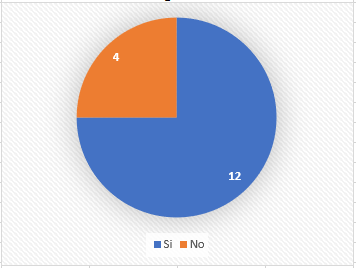
\includegraphics[width=0.55\textwidth]{Imagenes/Pregunta5.1.png}
    \caption{\label{fig: Pregunta5}Resultado de la pregunta cinco.}
\end{figure}

\textbf{6.  ¿El sistema logra realizar una Rendición fiable? (Siempre, A veces, nunca)}

\begin{figure}[h!]
    \centering
    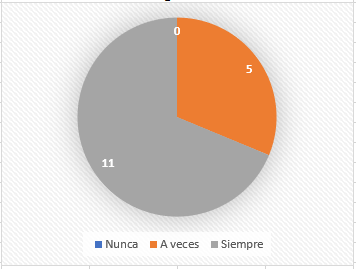
\includegraphics[width=0.55\textwidth]{Imagenes/Pregunta6.1.png}
    \caption{\label{fig: Pregunta6}Resultado de la pregunta seis.}
\end{figure}
	\section{Sección de preguntas sobre usabilidad e interfaz de usuario (En escala de 1 (En desacuerdo) a 5 (De acuerdo))}

\textbf{7.  ¿La aplicación es fácil de usar?}

\begin{figure}[h]
    \centering
    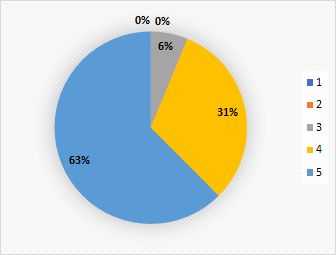
\includegraphics[width=0.5\textwidth]{Imagenes/Pregunta7.png}
    \caption{\label{fig: Pregunta7}Resultado de la pregunta siete.}
\end{figure}

\textbf{8.  ¿Se entiende cómo utilizar la aplicación sin necesidad de instrucciones?}

\begin{figure}[h]
    \centering
    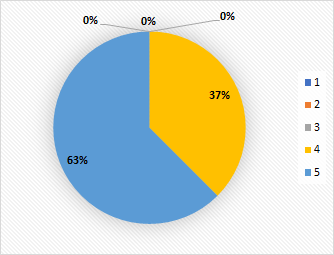
\includegraphics[width=0.5\textwidth]{Imagenes/Pregunta8.png}
    \caption{\label{fig: Pregunta8}Resultado de la pregunta ocho.}
\end{figure}

\newpage
\textbf{9. ¿La distribución de los elementos en la pantalla es adecuada?}

\begin{figure}[h]
    \centering
    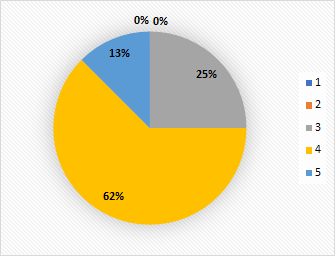
\includegraphics[width=0.55\textwidth]{Imagenes/Pregunta9.png}
    \caption{\label{fig: Pregunta9}Resultado de la pregunta nueve.}
\end{figure}

\textbf{10. ¿El proceso completo de realizar una Solicitud de Fondo por Rendir es claro?}

\begin{figure}[h]
    \centering
    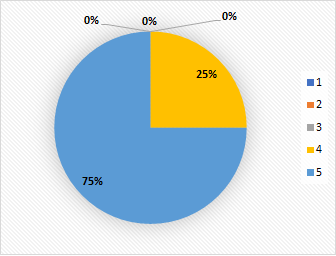
\includegraphics[width=0.55\textwidth]{Imagenes/Pregunta10.png}
    \caption{\label{fig: Pregunta10}Resultado de la pregunta diez.}
\end{figure}





%% fin
\end{document}

   

